\documentclass[conference]{IEEEtran}
\IEEEoverridecommandlockouts
% The preceding line is only needed to identify funding in the first footnote. If that is unneeded, please comment it out.
%Template version as of 6/27/2024
\usepackage{cite}
\usepackage{amsmath,amssymb,amsfonts}
\usepackage{algorithmic}
\usepackage{graphicx}
\usepackage{textcomp}
\usepackage{xcolor}
\usepackage{placeins}
	\usepackage{graphicx} % ở preamble
\def\BibTeX{{\rm B\kern-.05em{\sc i\kern-.025em b}\kern-.08em
		T\kern-.1667em\lower.7ex\hbox{E}\kern-.125emX}}
\begin{document}
	
	\title{Biometric Identification Through Auditory EEG Signatures}
	
	
	\author{\IEEEauthorblockN{1\textsuperscript{st} Ly Ngoc Vu}
		\IEEEauthorblockA{\textit{Faculty of Information Technology} \\
			\textit{Industrial University, HCMC, Vietnam}\\
			dezzhuge@gmail.com}
		\and
		\IEEEauthorblockN{2\textsuperscript{nd} Bui Thi Ngoc Tran}
		\IEEEauthorblockA{\textit{Faculty of Information Technology} \\
			\textit{Industrial University, HCMC, Vietnam}\\
			tranbui2907@gmail.com}
		\and
		\IEEEauthorblockN{3\textsuperscript{rd} Huynh Cong Bang}
		\IEEEauthorblockA{\textit{Faculty of Information Technology} \\
			\textit{Industrial University, HCMC, Vietnam}\\
			bang\_01036047@iuh.edu.vn}
		\and
		\IEEEauthorblockN{4\textsuperscript{th} Nguyen Minh Hanh}
		\IEEEauthorblockA{\textit{Faculty of Information Technology} \\
			\textit{Industrial University, HCMC, Vietnam}\\
			hanh\_01036046@iuh.edu.vn}
	}
	
	\maketitle
	
	\begin{abstract}
		Intelligent authentication systems for real-world deployment must be robust to noise, scalable to new users, and capable of operating under open-set conditions. However, many existing approaches remain constrained by closed-set assumptions and limited resilience to signal degradation, reducing their practical applicability. This research presents a noise-resilient open-set authentication framework that integrates adaptive signal enhancement with discriminative representation learning. A WaveNet-based denoising module, optimized using a scale-invariant signal-to-noise ratio objective, mitigates environmental and physiological noise. In contrast, a deep metric learning module built on ResNet backbones and angular margin-based losses learns a compact embedding space for reliable identity discrimination and unseen-user detection. Using brain-derived signals as a case study, the proposed framework achieves near-perfect identity retrieval performance and approximately 98\% accuracy in open-set recognition. Further analysis highlights the importance of jointly optimizing noise mitigation and embedding learning objectives in intelligent authentication systems. Overall, the proposed framework provides a scalable and deployable solution for secure authentication across intelligent sensing and biometric applications.
	\end{abstract}
	\begin{IEEEkeywords}
Biometric identification, EEG authentication, Open-set recognition, Deep metric learning, Signal enhancement.
	\end{IEEEkeywords}
	\section{Introduction}
	The rapid proliferation of intelligent systems in security-sensitive applications has intensified the demand for authentication mechanisms that are not only accurate but also robust, scalable, and adaptable to real-world conditions. Modern authentication systems are increasingly deployed in dynamic environments such as smart devices, wearable technologies, and cyber-physical systems, where signal quality, user populations, and operating conditions cannot be strictly controlled. As a result, intelligent authentication solutions must handle noisy inputs, accommodate newly encountered users, and operate reliably in open-set scenarios \cite{Fallahi2023, Yang2022, Zhang2017}.\\
	Traditional authentication approaches, including password-based methods and conventional biometric systems, face well-known limitations, such as security vulnerabilities, spoofing, and limited adaptability. While recent advances in machine learning and deep learning have significantly improved biometric authentication performance, many existing methods remain constrained by closed-set assumptions, under which all user identities are assumed to be known during training \cite{Fallahi2023, Yang2022, Zhang2017}. Such assumptions are unrealistic in practical deployments, where systems must continuously handle previously unseen users. Moreover, real-world sensory data are often corrupted by environmental and physiological noise, resulting in degraded performance and reduced reliability \cite{Alzahab2024, Fallahi2023}.\\
	To address these challenges, representation learning and deep metric learning have emerged as powerful paradigms for intelligent authentication. By learning discriminative embedding spaces that preserve semantic similarity, metric learning enables identity verification, retrieval, and open-set recognition within a unified framework \cite{Hadsell2006, Schroff2015,Wang2019,Deng2019}. However, the effectiveness of embedding-based authentication systems is highly sensitive to the quality of the input signal. In noisy conditions, poorly structured embeddings can significantly impair both discrimination accuracy and unseen-user detection, underscoring the need for robust signal enhancement mechanisms \cite{Fallahi2023,Alzahab2024}.\\
	In parallel, recent advances in deep neural architectures for signal enhancement have demonstrated strong potential to mitigate noise in complex, non-stationary signals. Models such as WaveNet have shown remarkable ability to learn signal structures directly from raw data, enabling adaptive denoising across diverse noise conditions\cite{vanDenOord2016}. Despite these advances, integrating noise-adaptive signal enhancement with discriminative representation learning for open-set authentication remains underexplored, particularly from a system-level perspective \cite{Fallahi2023,Yang2022}.\\
	This research addresses these gaps by proposing an intelligent authentication framework that jointly considers noise resilience and open-set recognition. The framework integrates a WaveNet-based adaptive denoising module with a deep metric-learning architecture built on ResNet backbones and angular-margin--based loss functions \cite{He2016,Deng2019,Wang2019}. By combining noise-aware signal enhancement with embedding-level discrimination, the proposed system is designed to operate reliably in realistic environments and scale to previously unseen users \cite{Hadsell2006,Schroff2015,Fallahi2023}. Using brain-derived signals as a representative case study, extensive experiments demonstrate that the proposed approach achieves high robustness, near-perfect identity retrieval, and strong open-set recognition performance \cite{Alzahab2024,Fallahi2023,Yang2022}. The results highlight the importance of jointly optimizing noise mitigation and representation learning objectives when designing deployable intelligent authentication systems \cite{Wang2019,Deng2019}.
	
	\section{Related work}
	Intelligent authentication systems have attracted growing attention as security requirements increase in dynamic and resource-constrained environments such as smart devices, wearable platforms, and cyber--physical systems. Traditional authentication mechanisms, including passwords and token-based methods, are prone to well-known security vulnerabilities. At the same time, conventional biometric systems based on facial images, fingerprints, or voice signals remain susceptible to spoofing attacks \cite{Fallahi2023}. As a result, learning-based authentication approaches have been widely investigated to enhance robustness and adaptability.\\
	Early learning-based authentication studies primarily focused on closed-set classification, assuming that all user identities are known during training. Using neural or physiological signals, Zhang \emph{et al.} employed attention-based recurrent neural networks to achieve high identification accuracy under controlled conditions \cite{Zhang2017}. Subsequent works extended this line of work by applying convolutional and Siamese network architectures to raw signal representations, demonstrating competitive performance while reducing reliance on handcrafted features \cite{Fallahi2023,Yang2022}. However, most of these approaches remain constrained by closed-set assumptions, limiting their scalability in real-world deployments.\\
	To address this limitation, open-set recognition has been increasingly explored in authentication systems. Metric learning has emerged as an effective paradigm for open-set authentication by learning embedding spaces in which identity similarity is preserved through distance relationships rather than fixed class assignments. Loss functions such as contrastive loss \cite{Hadsell2006} and triplet loss \cite{Schroff2015} have been widely adopted to improve discriminative representation learning. More recently, angular margin--based losses, including ArcFace, have demonstrated superior embedding compactness and inter-class separability, leading to improved stability in identity discrimination and retrieval tasks \cite{Deng2019}. Nevertheless, the effectiveness of metric learning--based authentication remains highly sensitive to input noise and signal variability.\\
	Robustness to noise is a critical challenge in practical authentication systems, as real-world signals are often corrupted by environmental interference and physiological artifacts \cite{Alzahab2024}. Traditional filtering and handcrafted feature extraction methods have been widely used to mitigate noise, but their performance is limited under complex, non-stationary conditions. Recent deep learning--based denoising approaches, particularly those capable of modeling temporal dependencies, have shown strong potential for adaptive noise suppression. Despite these advances, most existing studies treat signal enhancement and representation learning as independent components, without explicitly optimizing their interaction for open-set authentication.\\
	Brain-derived signals have also been explored as an alternative authentication modality due to their inherent uniqueness and resistance to spoofing. Prior studies have reported promising identification performance using both traditional machine learning and deep learning models \cite{Fallahi2023,Yang2022,Zhang2017}. However, these systems remain vulnerable to noise, session variability, and deployment constraints, and open-set operation is often insufficiently addressed \cite{Alzahab2024}. Additionally, ethical considerations around privacy and user consent are crucial when deploying brain-derived signal systems. Acknowledging these concerns can build trust with users by ensuring their data is handled with care, transparency, and in compliance with relevant regulations. By addressing these ethical aspects, the potential of brain-derived signals as a secure and reliable modality can be fully realized, anticipating stakeholders' concerns while reinforcing their value in authentication.\\
	In summary, although prior work has demonstrated the effectiveness of metric learning and noise suppression for authentication, there remains a lack of integrated frameworks that jointly address noise resilience, discriminative representation learning, and open-set recognition at the system level. This gap motivates the proposed approach. Unlike prior EEG biometric studies that rely on single-stage classification models, this work formulates EEG authentication as a two-stage learning problem, decoupling deep representation learning from identity discrimination via metric learning \cite{Hadsell2006,Schroff2015,Deng2019,Wang2019}. This design enables robust open-set authentication and superior generalization to unseen subjects.
	\section{Methodology}
	This study proposes a two-stage authentication framework that enhances robustness and open-set capability by explicitly decoupling noise mitigation from representation learning. The overall architecture consists of a noise-adaptive signal enhancement stage followed by a deep metric learning--based embedding stage, as illustrated in Fig.~\ref{fig:framework}.
	
	\begin{figure}[htbp]
		\centering
		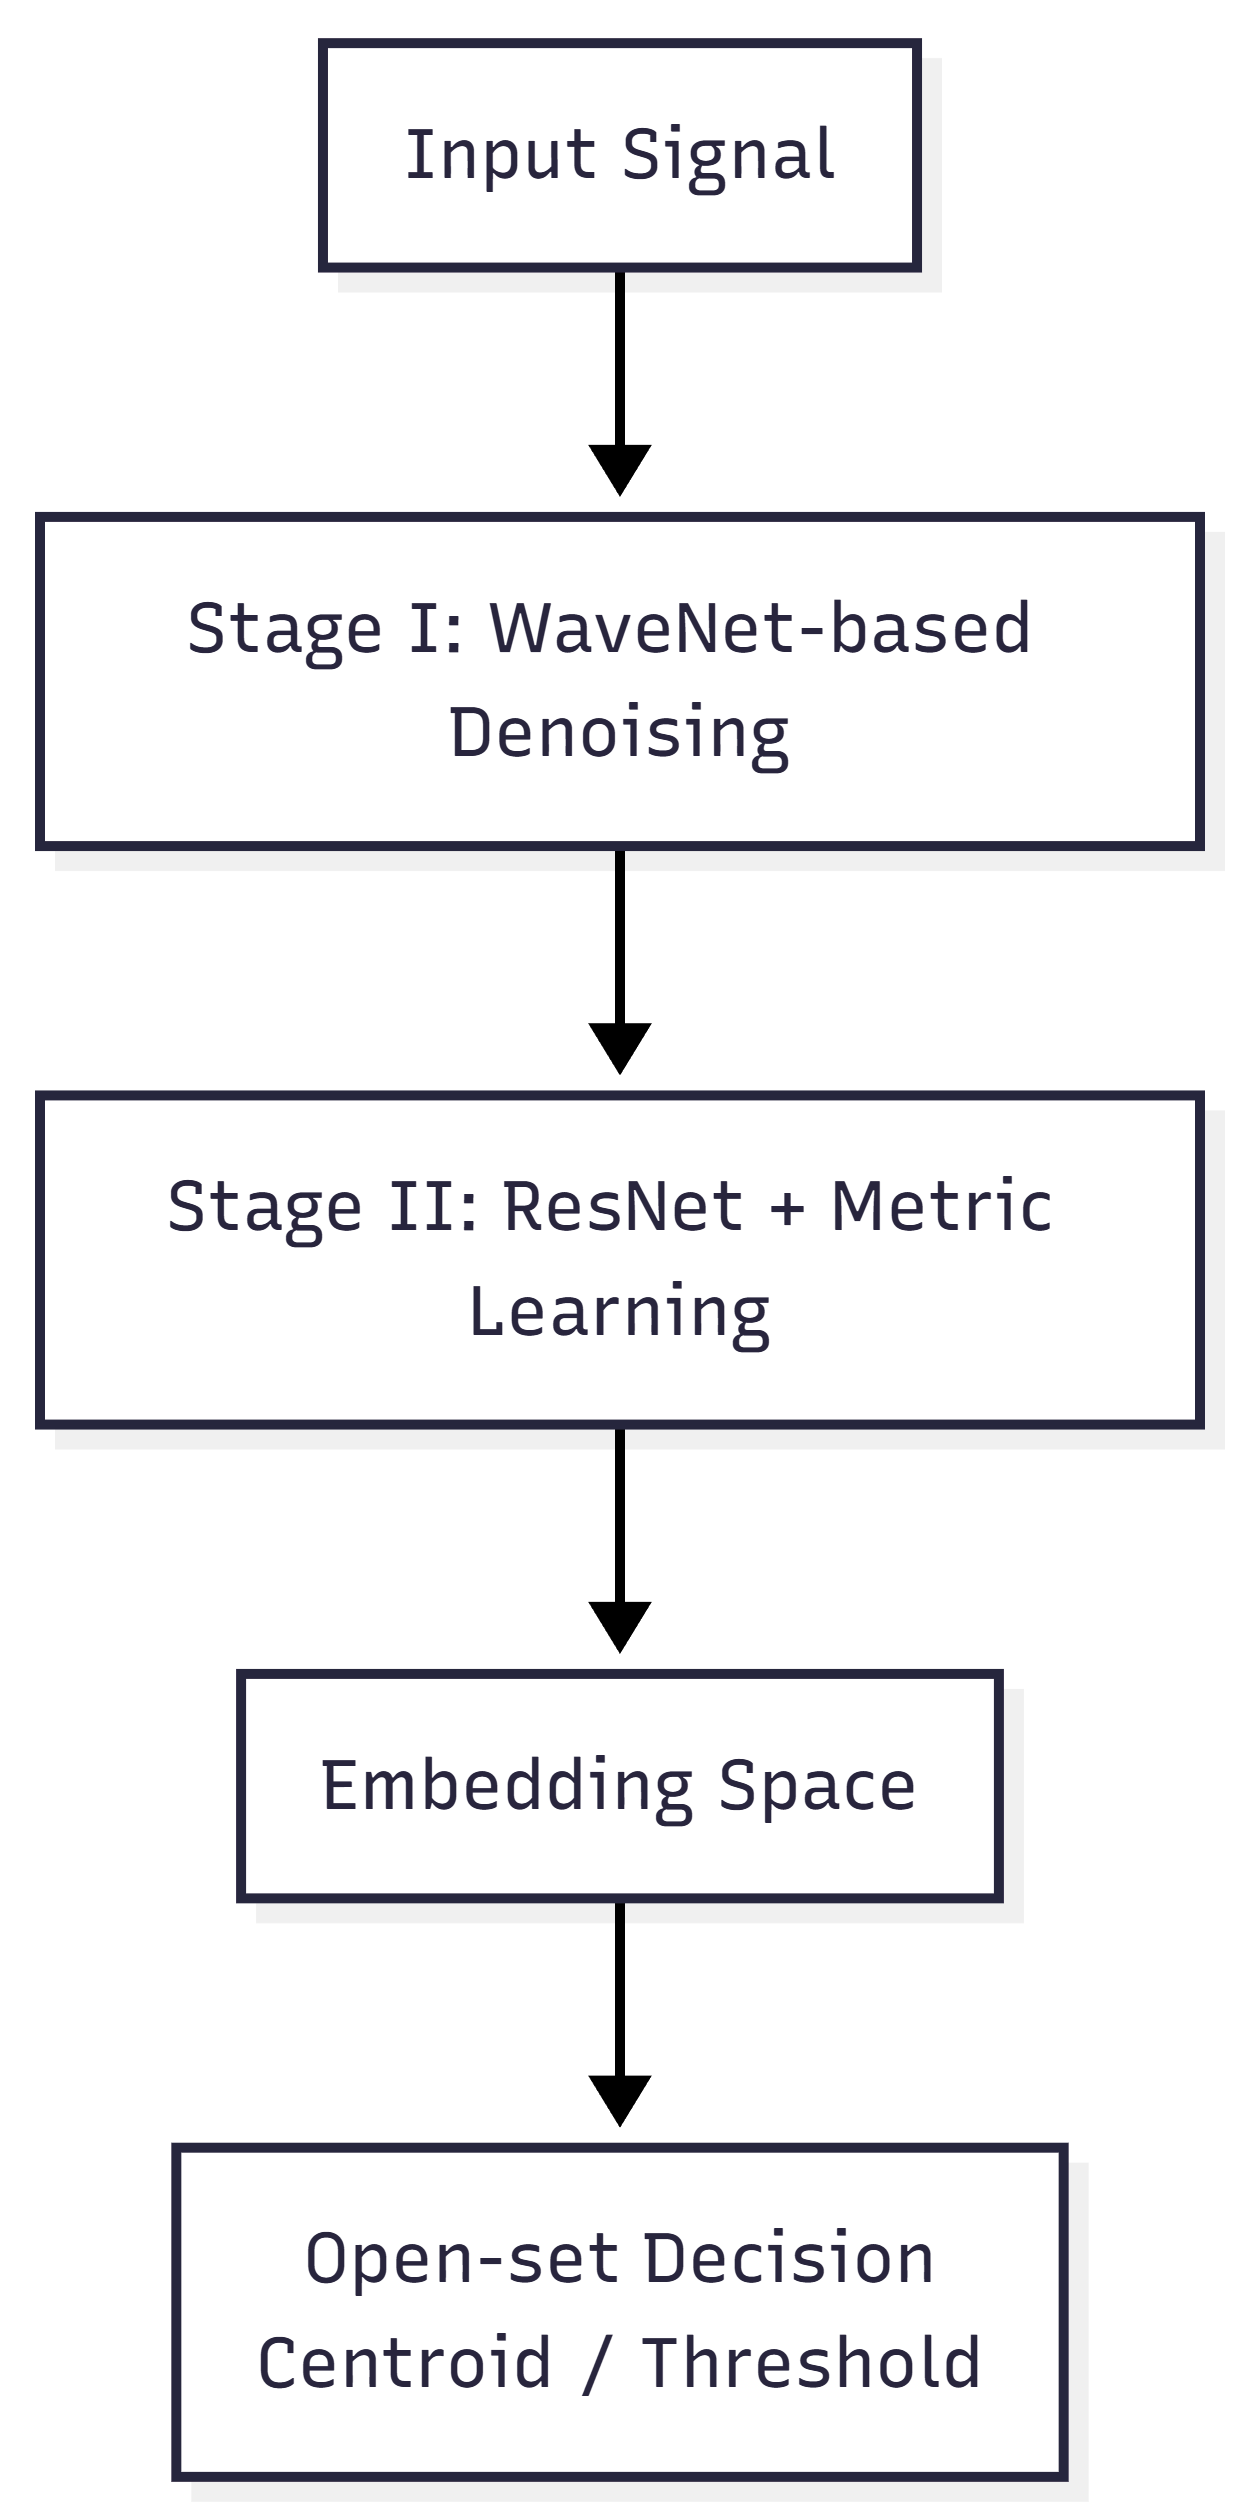
\includegraphics[width=0.7\linewidth]{./2stages.png}
		\caption{Overview of the proposed two-stage authentication framework.}
		\label{fig:framework}
	\end{figure}
	
	\subsection{Stage I: Noise-Adaptive Signal Enhancement}
\begin{figure*}[htbp]
	\centering
	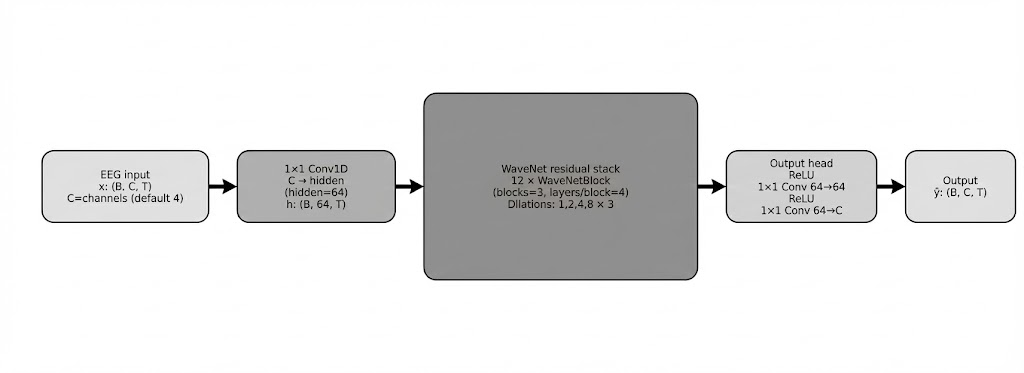
\includegraphics[width=0.8\textwidth]{wavenet_denoise_arch_en_notitle}
	\caption{WaveNetDenoiser architecture for EEG denoising.}
	\label{fig:wavenet-denoiser-arch}
\end{figure*}

	
	The first stage aims to mitigate environmental and physiological noise that commonly degrades real-world signals \cite{Alzahab2024}. A WaveNet-based denoising model is employed to learn a direct mapping from noisy inputs to cleaner signal representations \cite{vanDenOord2016}. The model is trained using a scale-invariant signal-to-noise ratio (SI-SNR) objective, which encourages faithful signal reconstruction while remaining insensitive to amplitude variations. By explicitly performing denoising before representation learning, this stage reduces noise-induced distortions and improves signal consistency across sessions and operating conditions. Fig.~\ref{fig:wavenet-denoiser-arch}\\
	\textbf{Noise synthesis and denoiser training.}
	To train Stage I, we construct paired samples $(x_{\text{noisy}}, x_{\text{clean}})$ using only subjects in $\mathcal{S}_{\text{train}}$.
	We define $x_{\text{clean}}$ as the EEG from dataset and generate
	$x_{\text{noisy}} = x_{\text{clean}} + \alpha n$, where $n$ is sampled from Gaussian / power-line / EMG noise
	and $\alpha$ is set to match a target SNR range.
	The WaveNet denoiser is optimized with the SI-SNR objective to recover $x_{\text{clean}}$ from $x_{\text{noisy}}$.
	
	\subsection{Stage II: Discriminative Representation Learning}
	In the second stage, denoised signals are processed by a deep metric learning model to learn identity-discriminative embeddings \cite{Hadsell2006,Schroff2015}. Residual convolutional neural networks (ResNet) are used as backbone architectures due to their stability and strong representation capacity \cite{He2016}. Angular margin--based loss functions are employed to enforce compact intra-class clustering and clear inter-class separation in the embedding space \cite{Deng2019}. In addition, general pair-weighted metric objectives (e.g., multi-similarity loss) can further improve embedding discrimination by leveraging multiple positive and negative relationships within a batch \cite{Wang2019}. This embedding-based formulation naturally supports open-set recognition, enabling the detection of unseen users based on distance to learned identity prototypes in the embedding space \cite{Hadsell2006,Schroff2015}.
	\section{Experimental Setup}
	\textbf{Dataset.} We used the publicly available \emph{Auditory Evoked Potential EEG--Biometric Dataset} from PhysioNet (2024), collected at the University of Chieti--Pescara, Italy~\cite{Alzahab2024}, for our experiments. This dataset consists of EEG recordings from 20 participants, each recorded over 12 sessions lasting approximately two minutes each, under two main conditions: resting-state (eyes open and eyes closed) and auditory stimulation. We selected this dataset because its structure allows examination of both inter- and intra-subject variability, which is critical for evaluating biometric authentication systems. During the auditory stimulation, subjects listened to native-language speech, foreign-language speech, and neutral sounds, presented through both in-ear and bone-conduction headphones. The use of these two headphone types is relevant because it introduces variability in auditory stimulus delivery methods, which may affect the resulting EEG responses and thus provides a means to assess the generalizability and robustness of biometric authentication. Furthermore, the combination of multiple types of auditory stimuli and different hardware enables us to simulate real-world heterogeneity in experimental conditions, providing insight into how such factors might influence authentication accuracy. The inclusion of multiple sessions introduces substantial inter-session variability, making this dataset well-suited for evaluating robustness and open-set authentication performance.
	Auditory stimulation elicits measurable evoked responses in EEG signals, forming subject-specific patterns across sessions. Such brain-derived signatures are inherently more difficult to spoof than conventional biometrics, but they are sensitive to noise and session variability.
	
	\textbf{Protocol and baselines.} EEG recordings were segmented into fixed-length epochs and divided into training and test sets using a subject-independent protocol, ensuring that test identities were not seen during training. We compared our proposed two-stage framework against several deep learning baselines, including recurrent models (LSTM and BiLSTM)~\cite{Hochreiter1997, Graves2005} and single-stage convolutional architectures trained on raw signals without explicit denoising~\cite{Zhang2017, Fallahi2023, Yang2022}. All methods were trained under identical conditions to ensure fair comparison. Performance was evaluated using Precision@1 (P@1) for identity retrieval and TAR (\%) for open-set acceptance of known users~\cite{Hadsell2006, Schroff2015}.
	

	\textbf{Open-set protocol (subject-independent).}
	We adopt a subject-independent evaluation where the training and evaluation subject sets are disjoint:
	$\mathcal{S}_{\text{train}} \cap \mathcal{S}_{\text{eval}}=\varnothing$.
	The embedding network $f(\cdot)$ is trained only on $\mathcal{S}_{\text{train}}$.
	
	\textbf{Enrollment.} From $\mathcal{S}_{\text{eval}}$, we define an enrolled set $\mathcal{S}_{\text{enroll}}$ and compute
	a prototype for each enrolled subject $c$ using enrollment epochs $\mathcal{E}_c$:
	$\mu_c=\frac{1}{|\mathcal{E}_c|}\sum_{x\in\mathcal{E}_c} f(x)$.
	The remaining subjects are treated as unknown:
	$\mathcal{S}_{\text{unknown}}=\mathcal{S}_{\text{eval}}\setminus\mathcal{S}_{\text{enroll}}$.
	
	\textbf{Decision rule.} For a query $x$, we compute $z=f(x)$ and
	$d^*=\min_{c\in\mathcal{S}_{\text{enroll}}}\|z-\mu_c\|_2$.
	We accept the closest identity if $d^*\le \tau$; otherwise we reject as unknown.
	
	\textbf{Threshold calibration.} The threshold $\tau$ is calibrated without using test queries,
	using a held-out calibration split of enrolled subjects (e.g., separate sessions/epochs).
	We select $\tau$ either to meet a target FAR on the calibration set or as the $p$-th percentile of genuine distances.
	Once selected, $\tau$ is fixed for all test evaluations; each model is calibrated with the same procedure for fairness.
	
	
	\section{Results and Discussion}
	
	\begin{figure}[htbp]
		\centering
		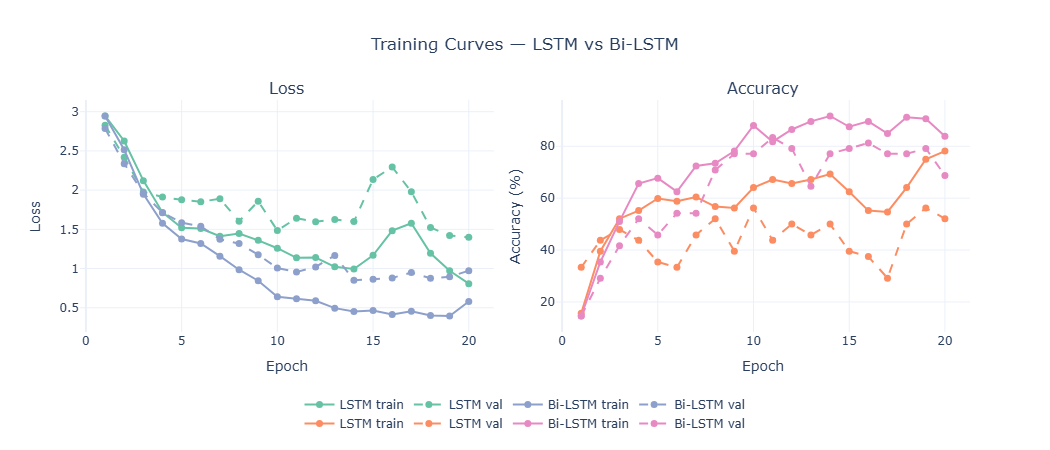
\includegraphics[width=0.7\linewidth]{./fig9}
		\caption{Performance comparison between single-stage recurrent baselines (LSTM and BiLSTM).}
		\label{fig:lstm_bilstm}
	\end{figure}
	
	Experimental results show that the proposed two-stage framework consistently outperforms single-stage deep learning baselines. As illustrated in Fig.~\ref{fig:lstm_bilstm}, recurrent models (LSTM/BiLSTM) provide competitive performance under clean conditions. Still, their reliability degrades under noise and session variability, which is consistent with the known sensitivity of temporal models to distribution shifts and corrupted inputs \cite{Hochreiter1997, Graves2005}.
	
	\subsection{Effect of Metric Learning Objectives}
	Table~\ref{tab:dml_resnet} compares different deep metric learning objectives on ResNet backbones. Across architectures, metric learning losses significantly improve discriminative embeddings compared with conventional closed-set formulations by explicitly optimizing distances in the embedding space \cite{Hadsell2006, Schroff2015}. In particular, multi-similarity loss and ArcFace achieve the strongest performance, indicating better intra-class compactness and inter-class separability \cite{Wang2019, Deng2019}. ResNet backbones are used due to their stable optimization and strong representational capacity \cite{He2016}.
	
	\begin{table}[htbp]
		\centering
		\caption{Performance comparison of deep metric learning losses on ResNet backbones.}
		\label{tab:dml_resnet}
		\begin{tabular}{l l c}
			\hline
			\textbf{Backbone} & \textbf{Loss Function} & \textbf{Accuracy (\%)} \\
			\hline
			ResNet-18 & Triplet Loss        & 97.89 \\
			ResNet-18 & Contrastive Loss    & 97.96 \\
			ResNet-18 & Multi-Similarity    & 98.67 \\
			ResNet-18 & ArcFace             & 98.60 \\
			\hline
			ResNet-34 & Triplet Loss        & 94.27 \\
			ResNet-34 & Contrastive Loss    & 98.07 \\
			ResNet-34 & Multi-Similarity    & \textbf{98.84} \\
			ResNet-34 & ArcFace             & 98.81 \\
			\hline
			ResNet-50 & Triplet Loss        & 92.76 \\
			ResNet-50 & Contrastive Loss    & 97.65 \\
			ResNet-50 & Multi-Similarity    & 98.52 \\
			ResNet-50 & ArcFace             & 98.56 \\
			\hline
		\end{tabular}
	\end{table}
	
	Overall, the proposed approach maintains near-perfect identity retrieval performance (P@1) and achieves approximately 98\% open-set recognition accuracy, demonstrating strong generalization beyond the closed-set assumption commonly adopted in earlier EEG biometric systems \cite{Zhang2017,Fallahi2023,Yang2022}.
	
	\subsection{Robustness Under Noise and Ablation Study}
	Table~\ref{tab:two_stage_results} reports P@1 and SI-SNR across different noise types. The results indicate that the framework remains stable under Gaussian, power-line, and EMG noise, suggesting that explicit enhancement improves downstream embedding discrimination. (Note that SI-SNR is included as a reconstruction-oriented indicator of denoising quality \cite{Luo2018}.)
	
	\begin{table}[htbp]
		\centering
		\caption{Performance of the proposed two-stage framework under different noise conditions.}
		\label{tab:two_stage_results}
		\begin{tabular}{l l c c}
			\hline
			\textbf{Noise} & \textbf{Model} & \textbf{P@1} & \textbf{SI-SNR (dB)} \\
			\hline
			Gaussian   & ResNet-34 + Multi-Similarity & 0.9380 & 12.62 \\
			Gaussian   & ResNet-18 + Multi-Similarity & \textbf{0.9424} & 12.61 \\
			Gaussian   & ResNet-34 + ArcFace          & 0.9336 & 12.69 \\
			\hline
			Power-line & ResNet-34 + Multi-Similarity & 0.9815 & 35.55 \\
			Power-line & ResNet-18 + Multi-Similarity & \textbf{0.9842} & 34.09 \\
			Power-line & ResNet-34 + ArcFace          & 0.9806 & 35.89 \\
			\hline
			EMG        & ResNet-34 + Multi-Similarity & \textbf{0.9762} & 14.18 \\
			EMG        & ResNet-18 + Multi-Similarity & 0.9626 & 14.17 \\
			EMG        & ResNet-34 + ArcFace          & 0.9644 & 14.09 \\
			\hline
		\end{tabular}
	\end{table}
	
	To quantify the contribution of Stage~I, Table~\ref{tab:ablation_main} presents an ablation study comparing single-stage training versus the full two-stage pipeline under each noise condition. Removing the noise-adaptive enhancement module results in a consistent drop in P@1, indicating that denoising improves embedding stability and helps preserve the discriminative structure for unseen-user detection. These findings support the hypothesis that explicitly separating noise mitigation from representation learning yields a more robust and deployable authentication pipeline.
	

	\begin{table}[htbp]
		\centering
		\caption{Ablation study of the proposed two-stage framework under different noise conditions.}
		\label{tab:ablation_main}
		\resizebox{\columnwidth}{!}{%
			\begin{tabular}{l l l c c}
				\hline
				\textbf{Noise} & \textbf{Framework} & \textbf{Model} & \textbf{P@1} & \textbf{TAR (\%)} \\
				\hline
				Gaussian   & Single-stage & ResNet-34 + Multi-Similarity & 0.9331 & 95.38 \\
				Gaussian   & Two-stage    & ResNet-34 + Multi-Similarity & \textbf{0.9380} & 94.37 \\
				\hline
				Power-line & Single-stage & ResNet-34 + Multi-Similarity & 0.9692 & 95.38 \\
				Power-line & Two-stage    & ResNet-34 + Multi-Similarity & \textbf{0.9815} & 95.64 \\
				\hline
				EMG        & Single-stage & ResNet-34 + Multi-Similarity & 0.9666 & 95.25 \\
				EMG        & Two-stage    & ResNet-34 + Multi-Similarity & \textbf{0.9762} & 95.51 \\
				\hline
			\end{tabular}%
		}
	\end{table}
	
	From a system-level perspective, the proposed two-stage design enables targeted optimization of enhancement and embedding objectives, improving interpretability and robustness in realistic conditions. This is particularly important for EEG-based authentication, where session variability and non-stationary noise frequently degrade performance \cite{Alzahab2024,Fallahi2023,Yang2022}.
	
	
	\section{Conclusion}
	This research presented a two-stage intelligent authentication framework that integrates adaptive noise mitigation with deep metric learning-based representation learning. By explicitly decoupling denoising from identity discrimination, the proposed approach enhances robustness, scalability, and open-set recognition. Experimental results demonstrate that the framework outperforms conventional single-stage deep learning models, achieving strong performance in identity retrieval and unseen-user detection. The proposed design offers a practical and deployable solution for secure authentication and can be extended to other intelligent sensing and biometric applications.
	\begin{thebibliography}{00}
		\bibitem{Fallahi2023}
		M.~Fallahi, T.~Strufe, and P.~Arias-Cabarcos,
		``BrainNet: Improving Brainwave-Based Biometric Recognition with Siamese Networks,''
		in \emph{Proc. IEEE PerCom}, 2023, pp.~53--60.
		
		\bibitem{Yang2022}
		H.~Yang, W.~Zheng, Y.~Zhang, and B.~L.~Lu,
		``EEG Authentication Based on Deep Learning of Triplet Loss,''
		\emph{Neural Network World}, vol.~32, no.~5, pp.~269--283, 2022.
		
		\bibitem{Zhang2017}
		X.~Zhang, L.~Yao, S.~S.~Kanhere, Y.~Liu, T.~Gu, and K.~Chen,
		``MindID: Person Identification from Brain Waves through Attention-Based Recurrent Neural Network,''
		arXiv:1711.06149, 2017.
		
		
		\bibitem{Alzahab2024}
		N.~A.~Alzahab \emph{et al.},
		``Auditory Evoked Potential Electroencephalography-Biometric Dataset,''
		\emph{Data in Brief}, vol.~57, p.~111065, 2024.
		
		\bibitem{Hadsell2006}
		R.~Hadsell, S.~Chopra, and Y.~LeCun,
		``Dimensionality Reduction by Learning an Invariant Mapping,''
		in \emph{Proc. IEEE CVPR}, 2006, pp.~1735--1742.
		
		\bibitem{Schroff2015}
		F.~Schroff, D.~Kalenichenko, and J.~Philbin,
		``FaceNet: A Unified Embedding for Face Recognition and Clustering,''
		in \emph{Proc. IEEE CVPR}, 2015, pp.~815--823.
		
		\bibitem{Deng2019}
		J.~Deng, J.~Guo, N.~Xue, and S.~Zafeiriou,
		``ArcFace: Additive Angular Margin Loss for Deep Face Recognition,''
		in \emph{Proc. IEEE/CVF CVPR}, 2019, pp.~4690--4699.
		
		\bibitem{Wang2019}
		X.~Wang \emph{et al.},
		``Multi-Similarity Loss with General Pair Weighting for Deep Metric Learning,''
		in \emph{Proc. IEEE/CVF CVPR}, 2019, pp.~5022--5030.
		
		\bibitem{Hochreiter1997}
		S.~Hochreiter and J.~Schmidhuber,
		``Long Short-Term Memory,''
		\emph{Neural Computation}, vol.~9, no.~8, pp.~1735--1780, 1997.
		
		\bibitem{Graves2005}
		A.~Graves and J.~Schmidhuber,
		``Framewise Phoneme Classification with Bidirectional LSTM,''
		\emph{Neural Networks}, vol.~18, no.~5--6, pp.~602--610, 2005.
		
		\bibitem{He2016}
		K.~He, X.~Zhang, S.~Ren, and J.~Sun,
		``Deep Residual Learning for Image Recognition,''
		in \emph{Proc. IEEE CVPR}, 2016, pp.~770--778.
		
		\bibitem{Davies1979}
		D.~L.~Davies and D.~W.~Bouldin,
		``A Cluster Separation Measure,''
		\emph{IEEE Trans. PAMI}, vol.~1, no.~2, pp.~224--227, 1979.
		
		\bibitem{Luo2018}
		Y.~Luo and N.~Mesgarani,
		``TasNet: Time-Domain Audio Separation Network for Real-Time, Single-Channel Speech Separation,''
		in \emph{Proc. IEEE ICASSP}, 2018, pp.~696--700, doi: 10.1109/ICASSP.2018.8462116.
		
		\bibitem{vanDenOord2016}
		A.~van~den~Oord \emph{et al.},
		``WaveNet: A Generative Model for Raw Audio,''
		arXiv:1609.03499, 2016.
	\end{thebibliography}
	
\end{document}
